\chapter{Defining a New Workload Model}

In order to improve on the homogenous, no startup-cost, workload model used in related work, we will first conduct power measurements on a sample program, and then use that information for the new model.

\section{Power Measurements on Machine Learning Jobs}
\label{sec:power_measurements}

\paragraph{The test environment}

The experiments were run on my personal computer, the components of that are listed via the \emph{hwlist} tool, with some columns and rows being redacted for brevity:

The experiments are run on a personal computer, its specification being outlined in Table \ref{tab:measurement_environment}, the values being determined with the \verb|hwlist| and \verb|lshw| commands.

\begin{table}[h!]
    \centering
    \begin{tabular}{|c|c|}
    \hline
        Operating system & Ubuntu 24.04 LTS \\ \hline
        Kernel & Linux 6.8.0-39-generic \\ \hline
        CPU & AMD Ryzen 5 1600X Six-Core Processor \\ \hline
        Memory & 16GiB \\ \hline
        GPU & GeForce GTX 1070 \\ \hline
    \end{tabular}
    \caption{Environment parameters of the power measurements}
\label{tab:measurement_environment}
\end{table}

\paragraph{Measurement tool}

As outlined in Chapter \ref{chap:backgroud}, multiple measurement options exist. 
As the HPI has the \emph{Microchip MCP39F511N Power Monitor (henceforth called MCP)} on-site, they will be used as a physical measurement device.
The MCP is placed between the device to test and the wall-mounted power supply. A picture of it can be found in figure \ref{fig:mcp}. It can report the current power consumption in 10 mW steps, each 5ms.

\begin{figure}
    \centering
    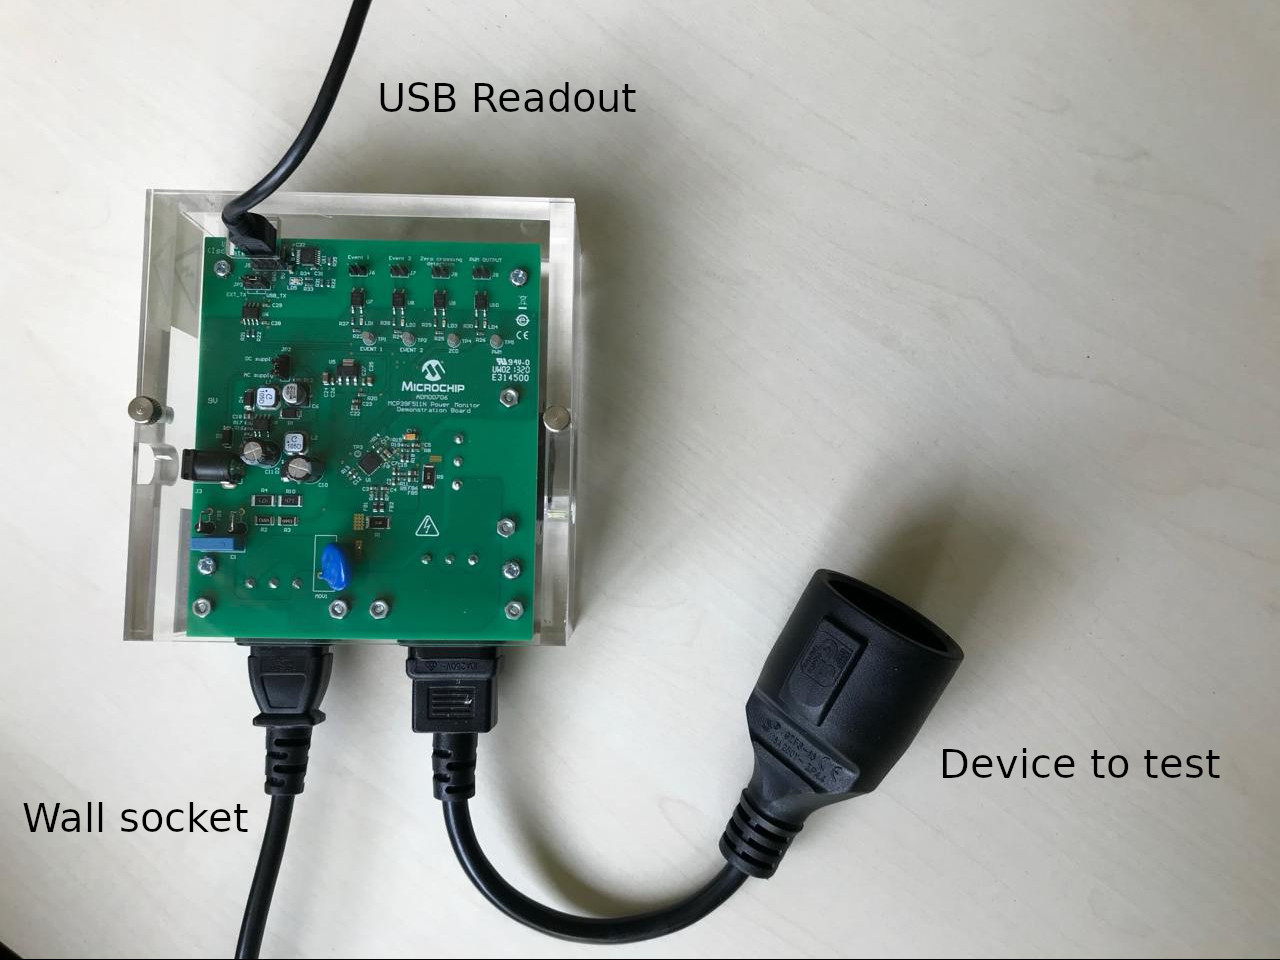
\includegraphics[width=200px]{images/mcp_graphic_design_is_my_passion.jpg}
    \caption[short]{The measurement tool we used. It can be inserted between a devices power supply and the wall socket. The encasing is not fully closed, so care needs to be taken not to touch any exposed contacts.}
    \label{fig:mcp}
\end{figure}

\todo{I could include an extra paragraph on why the MCP is cool, and what it does differently, perhaps. Was there anything cool? I vaguely remember some measurement devices having two capacitors to more accurately determine usage}

The software used for reading out MCP data is \emph{pinpoint}\cite{kohler_pinpoint_2020}.

\paragraph{Benchmark}

Machine learning (ML) was used as the main motivation for suspend \& resume scheduling in the related works\cite {wiesner_lets_2021} and thus was also chosen by us to be measured and modeled. 

The concrete model and framework are secondary to our measurement. In our case, a small model\webcite{web_distilbertdistilroberta-base_2024} is chosen to have fewer data points for processing, as well as faster iterations on the measurement script. 

There is a vast amount of machine learning frameworks. 
For a high-level model, the feature set of the framework only needed to support checkpointing, resuming, and some basic form of logging. 
A glance at the documentation of popular frameworks such as \emph{torch}, \emph{tensorflow}, and \emph{huggingface} shows that these features are commonly supported. 

With not much bias towards any framework, huggingface was chosen.
The huggingface trainer supports callbacks, we modified a given ML script to also log timestamped events when a training iteration, for example, starts or ends. 
These events are then saved into another \verb|.csv| file for each experiment.

\paragraph{Conducted Experiments}

A script \verb|measure_roberta.sh| was used to execute each experiment. 
On a high-level view, the following experiments were conducted: 

\begin{enumerate}
    \item \label{experiment:full}Run the whole program from start to finish
    \item \label{experiment:partial_checkpointed}Run it partially, checkpointing after some step, sleeping, and resuming from that step
    \item \label{experiment:partial_checkpointed_aborted}Run it partially, checkpointing after some step but aborting before the next checkpoint. Then resume as above.
    \item \label{experiment:startup_only}Run only the startup phase up until the ML would start
    \item \label{experiment:baseline}Do nothing, measure the system at rest
\end{enumerate}

Experiment \ref{experiment:full} gives a baseline for what the job looks like without suspend \& resume. Numbers \ref{experiment:partial_checkpointed} and \ref{experiment:partial_checkpointed_aborted} would be used to determine the overhead of checkpointing the job. \ref{experiment:startup_only} would be used to validate the other ones. The last experiment is necessary to determine the baseline energy consumption of the environment.

To execute these experiments inside a repeatable bash script, additional command line parameters were added to the program. 
For example, a boolean parameter \verb|--resume_from_checkpoint| and an integer parameter \verb|--stop_after_epoch| are used for experiment \ref{experiment:full} to \ref{experiment:partial_checkpointed}. 
The way of conducting experiment \ref{experiment:startup_only} was to copy the script, and delete everything after the imports.

\paragraph{Creating repeatable measurements}

As this is being run on standard hardware on a standard operating system, all experiments are subject to noise. 
For example, \emph{Dynamic frequency and voltage scaling (DFVS)}, the OS technique of increasing CPU "speeds" according to usage adds power in an uncontrolled way. Also, background tasks may happen \emph{randomly}, increasing power usage. 

Thus, for the testing, any foreground apps are closed. We also used the Linux tool \verb|cpupower|, as shown in the snippet below, to set the CPU frequency to a set value of 3.6 GHz, which is the maximum frequency:

\begin{minipage}{\linewidth}
\begin{lstlisting}[language=bash, frame=single, numbers=none, caption={Used operating system information}, basicstyle=\ttfamily]
    MINFREQ=$(cpupower frequency-info --hwlimits | sed -n '1d;p' \
        | awk '{print $1}')
    MAXFREQ=$(cpupower frequency-info --hwlimits | sed -n '1d;p' \
        | awk '{print $1}')
    
    cpupower frequency-set --min ${MAXFREQ} &>/dev/null
    cpupower frequency-set --max ${MAXFREQ} &>/dev/null

    # ... conduct experiments

    cpupower frequency-set --min ${MINFREQ} &>/dev/null
    cpupower frequency-set --max ${MAXFREQ} &>/dev/null
\end{lstlisting}
\label{listing:setting_cpu_frequency}
\end{minipage}

As machine learning makes use of available GPUs, the frequency should also be similarly set to a defined value. 
NVIDIA provides a guide on how to do so\footnote{\url{developer.nvidia.com/blog/advanced-api-performance-setstablepowerstate}}.
Our used GPU, the NVIDIA GTX 1070, is not capable of fixing the frequency as of the time of conducting these experiments. 
While it is supposed to be possible, there seems to currently be driver issue preventing this.\webcite{web_powerlimitissue}
Thus, the frequency of the GPU was not fixed. 
To reduce the effect of frequency scaling here, the time between experiments was increased generously so that any impact from such scaling reoccurs throughout each run, reducing dependencies between runs.

During the training, data is downloaded and saved, which is however deleted before the next experiment. 
The Python process is also not kept between runs, forcing a uniform load of any libraries.

\paragraph{Conducting each experiment}

Each experiment was re-run 10 times. Between each run, there is a \verb|sleep| period of 10 seconds and one of two minutes in the partial executions. 
Additionally, \verb|pinpoint|'s feature of measuring before and after the actual program-to-test would be used. 
This leads to a period of 30 seconds being measured around the program execution. 
Plotting these additional time frames gives a quick visual indicator of whether experiments are sufficiently isolated from each other, ergo when the power draw is at the baseline as the actual program starts. As some data being downloaded and persisted during the execution of the ML, before each run, that data is removed.

\paragraph{Collected data}

For each experiment, a named and timestamped folder is created in the \verb|/power-measurements| folder of my repository. Each folder then holds a \verb|.csv| with pinpoint's timestamped power measurements. 
The added timestamped logging is saved into another \verb|.csv|. 
On the way to the final measurements, we plot each experiment early and visually spot if there are any obvious errors or mistakes.

\paragraph{Determining the baseline power draw}

A sample run of the baseline experiment is shown in Figure \ref{fig:plot_baseline}.
The blue dots represent each data point. The red line is a smoothed Gaussian trend line with $\sigma = 2$. 
Dark-green vertical lines are the logged or derived "events" for each run. In this case, nothing happens, so it is only the start and end of \verb|sleep 120|. 
Notice how the trace starts 30 seconds before the start and continues for another 30 seconds because of the aforementioned \verb|pinpoint| feature.
Going further, these additional measurements will be redacted for brevity.

\begin{figure}
    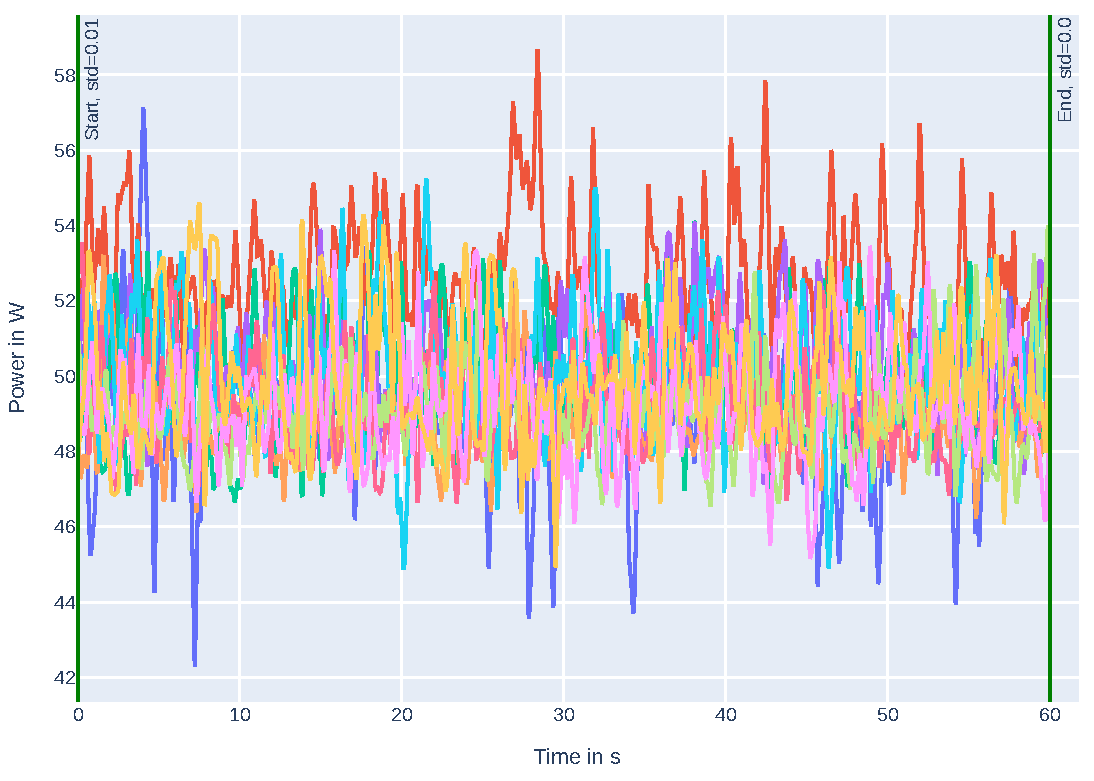
\includegraphics[width=\linewidth]{power-measurements/stacked_plots/sleep_0714.pdf}
    \caption{In the baseline experiment of measuring the system at rest, the average power draw is about 50 W. The black lines are Gaussian smoothed trend lines with $\sigma = 2$.}
    \label{fig:plot_baseline}
\end{figure}

Across all 10 runs, the average baseline power draw is calculated via the mean of all data points. This comes out as an average of 49.8 W with a standard deviation of 4.4 W.

The baseline power draw will be less interesting going further but will put perspective on the power draws of the other experiments. The standard deviation should give a broad idea of how much noise is in the system environment.

\paragraph{The non-interrupted run}

For the non-interrupted machine learning run, a sample run is provided in Figure \ref{fig:plot_full}. 
Figure \ref{fig:plot_full_stacked} shows the stacked trend lines of the 10 different runs.
For simplicity's sake, we refrained from doing a more elaborate statistical analysis of the different runs as the visual check of them being very similar seemed enough.

\begin{figure}
    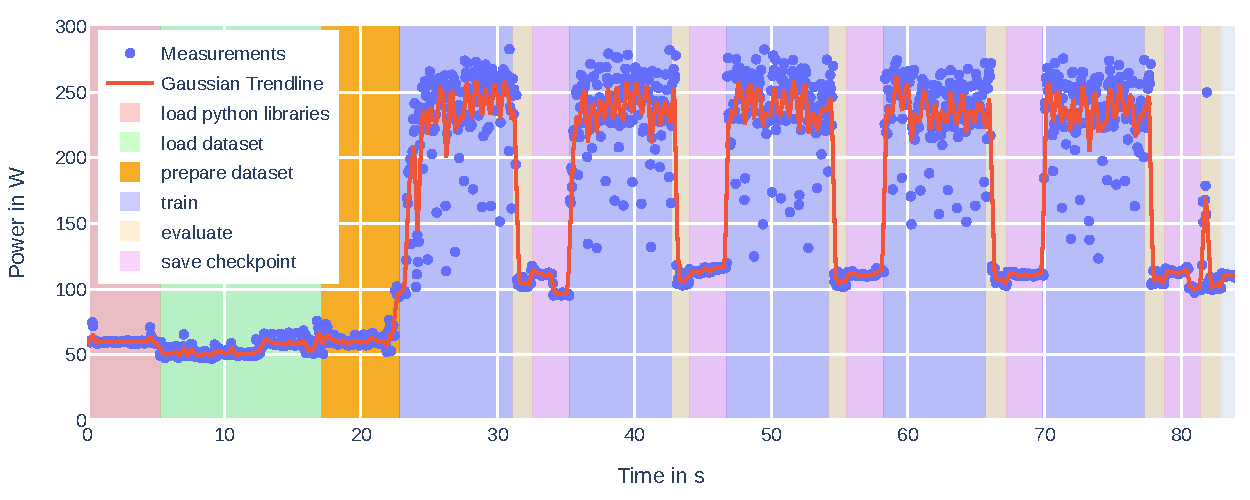
\includegraphics[width=\linewidth]{power-measurements/measurements_roberta_full_0714010405/plot.pdf}
    \caption{Sample run of the full run experiment, the background indicates the phase as determined by the added logging}
    \label{fig:plot_full}
\end{figure}

\begin{figure}
    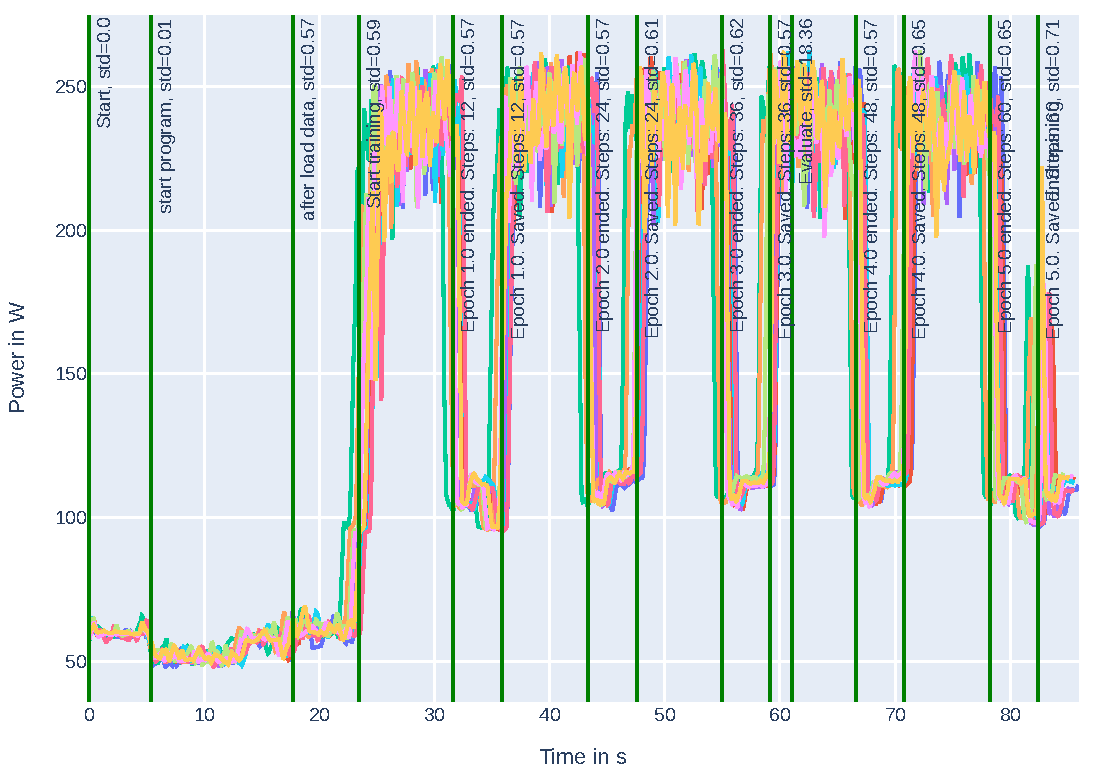
\includegraphics[width=\linewidth]{power-measurements/stacked_plots/roberta_full_0714.pdf}
    \caption{All full-run trend lines stacked. }
    \label{fig:plot_full_stacked}
\end{figure}

The main takeaways from these measurements are:

\begin{enumerate}
    \item There is a long (about 25\%) start-up phase, which is spent in starting Python, loading libraries, and loading data to disc.
    \item There are periodical work phases; a high-power training phase would be followed by low power evaluation\todo{Uhm, where did my evaluation phase markers go?? They are mushed together as they share a label} phase and a low-power checkpointing.
    \item A higher variance in measurements occurs during the training phases in comparison to the others.
\end{enumerate}

This already shows, that improvements upon the constant-power model used in \cite{wiesner_lets_2021} are possible. 
For example, in this case, the start-up phase has a much lower power-draw than the work-phase.

\paragraph{Results of the checkpoint and restore experiment}

Similarly to before, results will be discussed using the stacked plots \ref{fig:plot_partial_saved_stacked} and \ref{fig:plot_partial_saved_continue_stacked}; each run is plotted in the repository, however.

\begin{figure}
    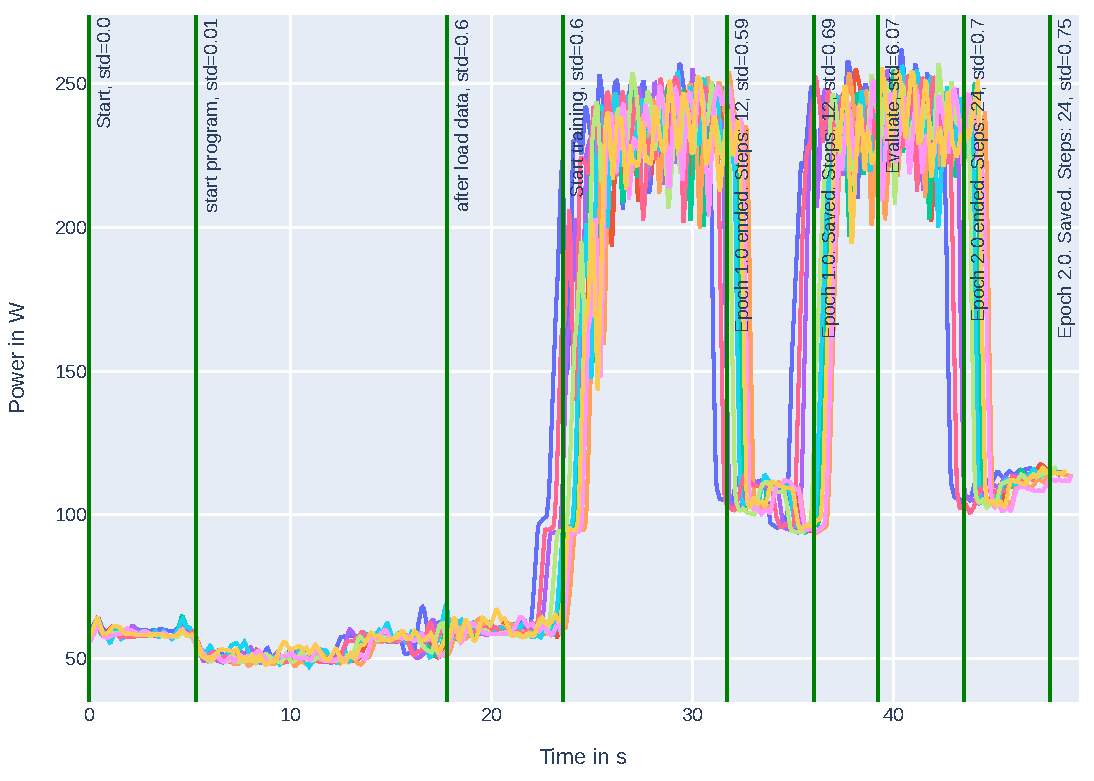
\includegraphics[width=\linewidth]{power-measurements/stacked_plots/roberta_stop_after_saving.pdf}
    \caption{Stacked trend lines of the experiment for stopping after the second epoch}
    \label{fig:plot_partial_saved_stacked}
\end{figure}

\begin{figure}
    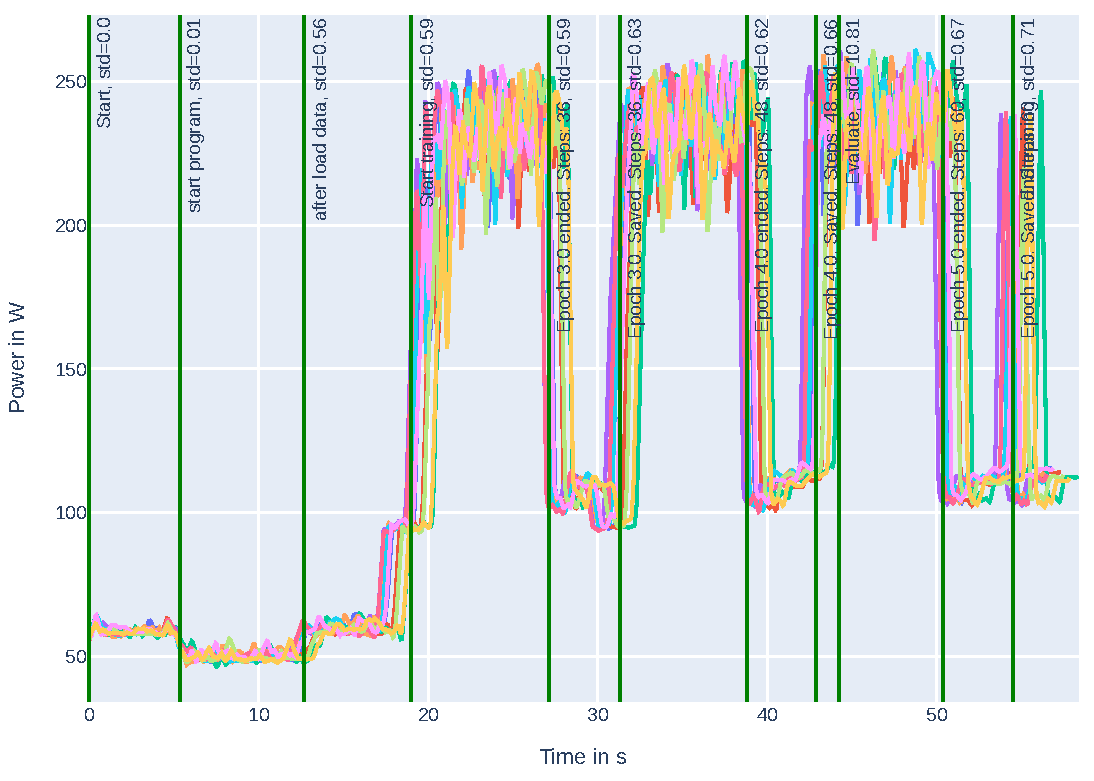
\includegraphics[width=\linewidth]{power-measurements/stacked_plots/roberta_continue_after_saving.pdf}
    \caption{Stacked trend lines of the experiment for continuing after the second epoch}
    \label{fig:plot_partial_saved_continue_stacked}
\end{figure}

Here we can observe that:

\begin{enumerate}
    \item The amount of work done is the same. 
    Similarly to the full-run experiment, the ML training still takes the full 5 epochs and has the same work-phases
    \item There is no overhead from checkpointing itself, as the checkpoints are being created regardless of them being resumed from later.
    \item Resuming the jobs results in an added start-up phase. This phase is slightly shorter by a few seconds than the ones in the full runs, likely due to not needing to download the dataset again.
\end{enumerate}

\paragraph{Results from checkpoint and resume with abort}

Unlike the previous experiment, where work is stopped as soon as a checkpoint is created, this time the program will be stopped just before a checkpoint is created (in this case just the second checkpoint would be saved). 
Ideally, this represents the maximum overhead from a suspend \& resume strategy. 

Again, the results are visualized in Figures \ref{fig:plot_partial_abort_stacked} and \ref{fig:plot_partial_abort_continue_stacked}. 
Attention should be paid that,

\begin{enumerate}
    \item The behavior of the repeated start-up phase is kept
    \item There is now a full additional training and evaluation phase added to the overall work, the aborted checkpoint is also repeated.
\end{enumerate}

While this may sound artificial, it could happen in environments where the interaction between the scheduler and the job is not well orchestrated, for example in an environment where jobs are stopped \emph{at random} like in a cloud spot instance. 
The average overhead from stopping the job at random vs. stopping after a checkpoint will likely fall at half the cost of an epoch.

\begin{figure}
    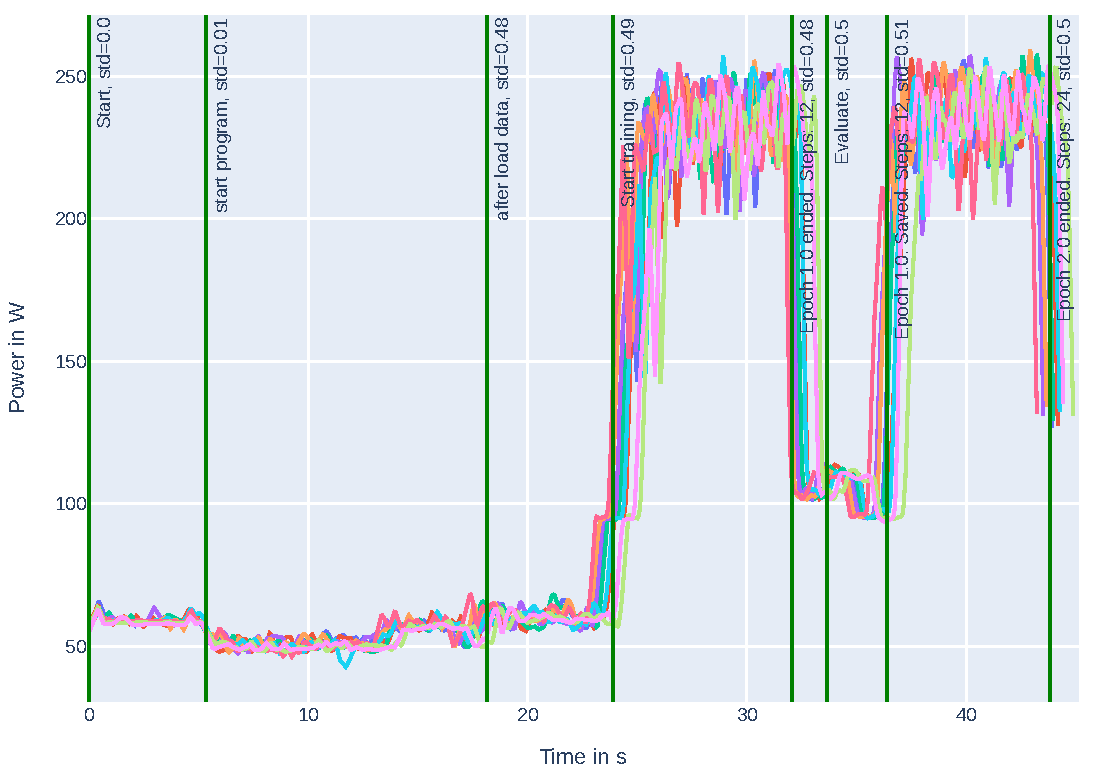
\includegraphics[width=\linewidth]{power-measurements/stacked_plots/roberta_stop_without_saving.pdf}
    \caption{Power draws of the ML up until stopping after epoch 2}
    \label{fig:plot_partial_abort_stacked}
\end{figure}

\begin{figure}
    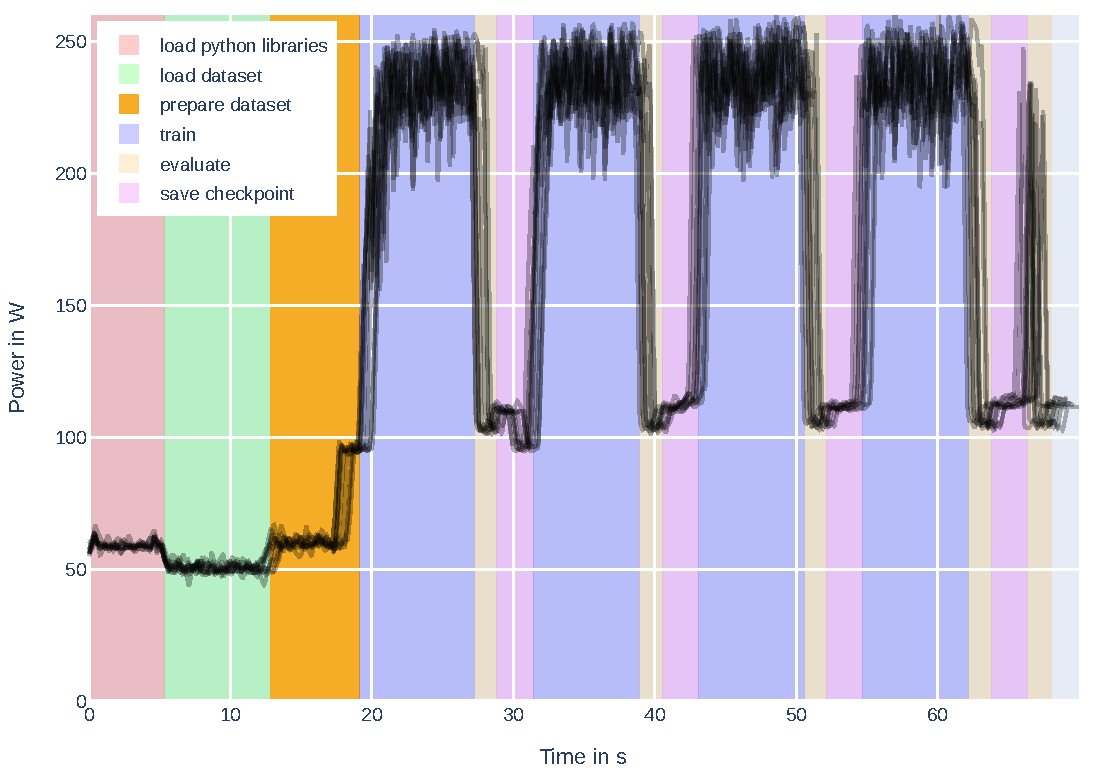
\includegraphics[width=\linewidth]{power-measurements/stacked_plots/roberta_continue_after_not_saving.pdf}
    \caption{Power draws after continuing from the second checkpoint}
    \label{fig:plot_partial_abort_continue_stacked}
\end{figure}

\paragraph{Calculating the energy costs of each run}

The energy costs of each experiment are contained in Table \ref{tab:experiment_overhead}.

\begin{table}[h!]
    \centering
    \begin{tabular}{|c|c|c|}
    \hline
        Experiment & average energy cost & standard deviation \\ \hline
        \ref{experiment:full}, whole run &  12.97 kJ & 0.04 \\ \hline
        \ref{experiment:partial_checkpointed}, suspend after checkpoint and resume &  13.94  kJ & 0.1 \\ \hline
        \ref{experiment:partial_checkpointed_aborted}, abort early and resume &  15.72 kJ & 0.07 \\ \hline
    \end{tabular}
    \caption{Environment parameters of the power measurements}
\label{tab:experiment_overhead}
\end{table}

\section{Introduction of \modelname} \label{sec:improving_the_model}

Now that we know what a high-level job looks like, we can pick it apart and reduce the real-world measurements of one program to a more generic model. 

Summarizing the findings from the previous paragraphs; it was shown that 

\begin{itemize}
    \item The given job has phases that have different power draws
    \item Checkpointing \& resuming carries overhead in the form of startup costs and possible wasted work.
\end{itemize}

The parameters for the improved job model are shown in the form of the Python implementation in Listing \ref{listing:model_python}.

\begin{minipage}{\linewidth}
\begin{lstlisting}[language=python, frame=single, numbers=none, caption={Python Model definition}, basicstyle=\ttfamily, label={listing:model_python}]
class Stawp(TypedDict):
    startup: List[Phase]
    work: List[Phase]
    
class Phase(TypedDict):
    name: str
    duration: float
    power: float
    is_checkpoint: NotRequired[bool]   
\end{lstlisting}
\end{minipage}

Some simplifications are made: the duration of each phase is well known and the power per phase is a constant. 
Phases can also be named for later reference.
These phases essentially define a step function, i.e. piecewise constant function.
Unlike a traditional step function, the start- and endpoints of each "piece" would be encoded implicitly by the previous phases.
Using these specifications, a simple time-to-power function can be defined, that looks up the input time and traverses the phases in order.

Initially, we considered allowing any expression instead of a constant value for power and then using Python's \verb|evaluate()| to e.g. allow a function-per-phase model.
In Section \ref{sec:checkpoint_resume_lp}, having a rather restrictive step function will be of advantage, however. \todo{Add some more explanation to this in that section}

The measurements that have been taken can now be fit into this new model. 
As each measurement point can be associated with a phase via the aforementioned added logging, the average of each phase-associated measurement is used to determine the model parameters. 
The durations of the phases are calculated similarly by taking the average time the logging occurred during the measurements.

Using this strategy on the 10 complete runs results in Figure \ref{fig:model_overlaid}, which shows the derived model in black with the previous Figure \ref{fig:plot_full} in less opacity. 
The startup phase looks well approximated, visually however there is some error during the work phases.
The training phases each have a high variance, which is not captured by the constant power approximation. After each training  phase, the power goes down seemingly linearly, which is also approximated by the constant.

One notable point, this model is a superset of the previous constant-no-overhead model used in the related work.
Previous jobs can be modeled with just one phase of work, resulting in constant power over its execution. Leaving the startup phases empty creates no overhead on resuming.

\todo{Should probably add the phase markers back in}
\begin{figure}
    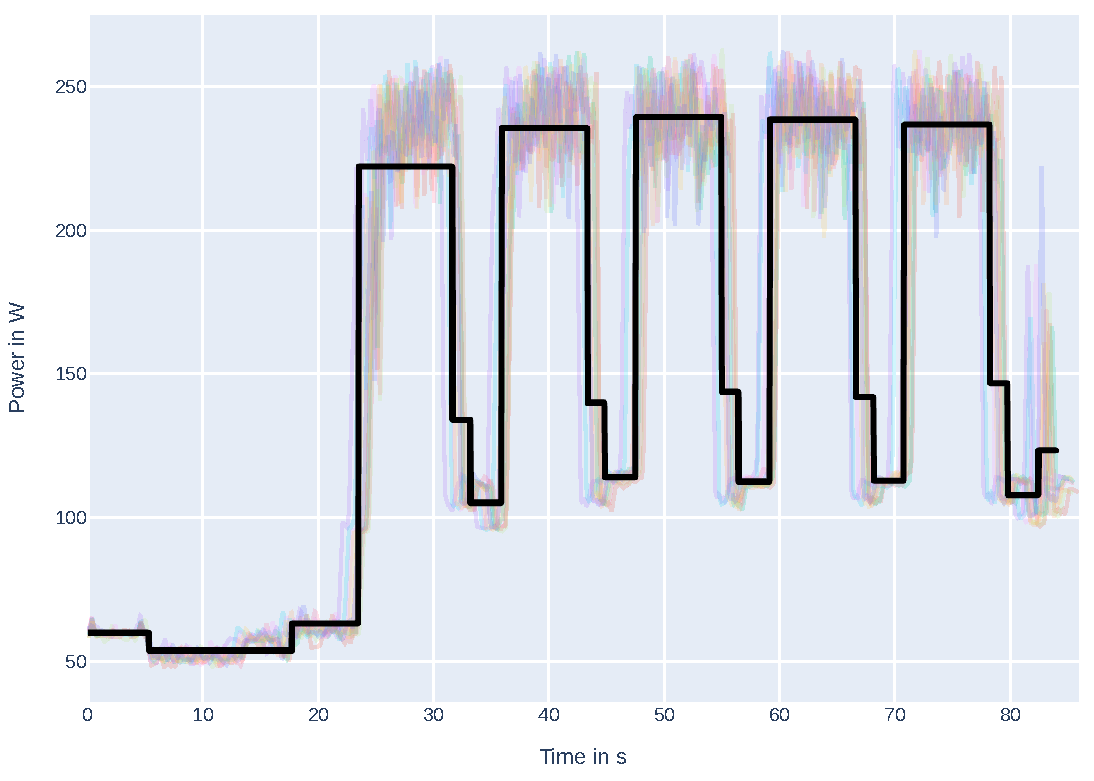
\includegraphics[width=\linewidth]{power-measurements/model_overlaid.pdf}
    \caption{Model of roberta.py (black) vs. the measured runs}
    \label{fig:model_overlaid}
\end{figure}

\paragraph{Model Error Analysis}

To analyze the error of this model, we cross-validated the power's RMSE and the total energy using \verb|scikit-learn|'s \verb|LeaveOneOut| strategy. 
The first one would give a measure of the model's accuracy on a short-time (sub-second) scale, the latter would  tell the long-time (whole job) scale accuracy of the model.

Each of the 10 runs would be taken as the ground truth while the other 9 would be used to create the model. 
The results are the following: the power between the prediction and remainder has an RSME of 39.3 W while the difference in total energy is calculated as -0.1 kJ. 

Interpreting this, it seems that the model performs poorly as a predictor of the exact power used at some time point as the RMSE is rather large (think of the maximum power drawn being about 250W). 
However, in the context of carbon-aware scheduling, this should not be too big of an issue as the time frames for carbon emissions are orders of magnitudes larger (\emph{electricitymaps} has a resolution of 1 hour for carbon emissions intensities). 
The high error likely comes from the high variance during the training phases which is not captured in the model.

The total energy predicted by the model is very close to the actual real-life experiment, this should mean that the total carbon calculated on the model should also be close to the carbon emitted by the real program.
